\documentclass[12pt]{article}%
\usepackage{amsfonts}
\usepackage{fancyhdr}
\usepackage{comment}
\usepackage[a4paper, top=2.5cm, bottom=2.5cm, left=2.2cm, right=2.2cm]%
{geometry}
\usepackage{times}
\usepackage{amsmath}
\usepackage{changepage}
\usepackage{amssymb}
\usepackage{graphicx}%
\setcounter{MaxMatrixCols}{30}
%\usepackage{hyperref}


%These tell TeX which packages to use.
\usepackage{array,epsfig}
\usepackage{amsmath}
\usepackage{amsfonts}
\usepackage{amssymb}
\usepackage{amsxtra}
\usepackage{amsthm}
\usepackage{mathrsfs}
\usepackage{color}





\usepackage{listings}
\usepackage{longtable}
\definecolor{codegreen}{rgb}{0,0.6,0}
\definecolor{codegray}{rgb}{0.5,0.5,0.5}
\definecolor{codepurple}{rgb}{0.58,0,0.82}
\definecolor{backcolour}{rgb}{0.96,0.96,0.94}
\lstdefinestyle{mystyle}{
	backgroundcolor=\color{backcolour},
	commentstyle=\color{codegreen},
	keywordstyle=\color{blue},
	numberstyle=\tiny\color{codegray},
	stringstyle=\color{codepurple},
	basicstyle=\footnotesize,
	breakatwhitespace=false,
	breaklines=true,
	captionpos=b,
	keepspaces=true,
	numbers=left,
	numbersep=5pt,
	showspaces=false,
	showstringspaces=false,
	showtabs=false,
	tabsize=2
}
\lstset{style=mystyle}

















%%%%%%%%% hyperref %%%%%%%%%%%%
\usepackage[pdftex,letterpaper=true,pdfpagelabels=true,pagebackref=true,bookmarks]{hyperref} 
% with basic options
% pagebackref=true provides links back from the References to the body text. This can cause trouble for printing.

%%%%%%%% cref cleverref %%%%%%%%%%%

% cref package must be loaded after hyperref !
\usepackage[noabbrev]{cleveref}




%Here I define some theorem styles and shortcut commands for symbols I use often
\theoremstyle{definition}
\newtheorem{defn}{Definition}
\newtheorem{thm}{Theorem}
\newtheorem*{thm*}{Theorem}
\newtheorem{cor}{Corollary}
\newtheorem*{rmk}{Remark}
\newtheorem{lem}{Lemma}
\newtheorem*{joke}{Joke}
\newtheorem{ex}{Example}
\newtheorem*{soln}{Solution}
\newtheorem{prop}{Proposition}




\newtheorem{sol}{Solution}


\newtheorem{theorem}{Theorem}
\newtheorem{acknowledgement}[theorem]{Acknowledgement}
\newtheorem{algorithm}[theorem]{Algorithm}
\newtheorem{axiom}{Axiom}
\newtheorem{case}[theorem]{Case}
\newtheorem{claim}[theorem]{Claim}
\newtheorem{conclusion}[theorem]{Conclusion}
\newtheorem{condition}[theorem]{Condition}
\newtheorem{conjecture}[theorem]{Conjecture}
\newtheorem{corollary}[theorem]{Corollary}
\newtheorem{criterion}[theorem]{Criterion}
\newtheorem{definition}[theorem]{Definition}
\newtheorem{example}[theorem]{Example}
\newtheorem{exercise}[theorem]{Exercise}
\newtheorem{lemma}[theorem]{Lemma}
\newtheorem{notation}[theorem]{Notation}
\newtheorem{problem}[theorem]{Problem}
\newtheorem{proposition}[theorem]{Proposition}
\newtheorem{remark}[theorem]{Remark}
\newtheorem{solution}[theorem]{Solution}
\newtheorem{summary}[theorem]{Summary}
%\newenvironment{proof}[1][Proof]{\textbf{#1.} }{\ \rule{0.5em}{0.5em}}

\newcommand{\Q}{\mathbb{Q}}
\newcommand{\R}{\mathbb{R}}
\newcommand{\C}{\mathbb{C}}
\newcommand{\Z}{\mathbb{Z}}


% operators
\DeclareMathOperator{\rank}{{rank}}
\DeclareMathOperator{\argmin}{{argmin}}
\DeclareMathOperator{\argmax}{{argmax}}
\DeclareMathOperator{\flatt}{{flat}}
\DeclareMathOperator{\sym}{{sym}}
\DeclareMathOperator{\sgn}{sgn}
\DeclareMathOperator{\conv}{conv}
\DeclareMathOperator{\env}{env}
\DeclareMathOperator{\dist}{dist}
\DeclareMathOperator{\epi}{epi}
\DeclareMathOperator{\Id}{Id}
\DeclareMathOperator{\dom}{dom}
\DeclareMathOperator{\cl}{cl}
\DeclareMathOperator{\Normal}{Normal}


% matrices
\newcommand{\bbm}{\begin{bmatrix}}
\newcommand{\ebm}{\end{bmatrix}}
\newcommand{\bem}{\begin{pmatrix}}
\newcommand{\eem}{\end{pmatrix}}

% parentheses
%\newcommand{\l[}{\left[}
%\newcommand{\r]}{\right]}
%\newcommand{\l(}{\left(}
%\newcommand{\r)}{\right)}

% 
\def\<{\langle}
\def\>{\rangle}

\usepackage{cite}



%%%%%%%%%%%% Mathcal{ } %%%%%%%
%%%%%%%%%%%%%%%%%%%%%%%%%%%%%%%
\newcommand{\cA}{{\mathcal A}}
\newcommand{\cB}{{\mathcal B}}
\newcommand{\cC}{{\mathcal C}}
\newcommand{\cD}{{\mathcal D}}
\newcommand{\cE}{{\mathcal E}}
\newcommand{\cF}{{\mathcal F}}
\newcommand{\cG}{{\mathcal G}}
\newcommand{\cDQ}{{\mathcal {DQ}}}
\newcommand{\cH}{{\mathcal H}}
\newcommand{\cI}{{\mathcal I}}
\newcommand{\cJ}{{\mathcal J}}
\newcommand{\cK}{{\mathcal K}}
\newcommand{\cL}{{\mathcal L}}
\newcommand{\cM}{{\mathcal M}}
\newcommand{\cN}{{\mathcal N}}
\newcommand{\cO}{{\mathcal O}}
\newcommand{\cP}{{\mathcal P}}
\newcommand{\cQ}{{\mathcal Q}}
\newcommand{\cR}{{\mathcal R}}
\newcommand{\cS}{{\mathcal S}}
\newcommand{\cT}{{\mathcal T}}
\newcommand{\cDP}{{\mathcal {DP}}}
\newcommand{\cU}{{\mathcal U}}
\newcommand{\cV}{{\mathcal V}}
\newcommand{\cW}{{\mathcal W}}
\newcommand{\cX}{{\mathcal X}}
\newcommand{\cY}{{\mathcal Y}}
\newcommand{\cZ}{{\mathcal Z}}

%%%%%%%%%%%% Mathbb{ } %%%%%%%%
%%%%%%%%%%%%%%%%%%%%%%%%%%%%%%%
\newcommand{\bA}{{\mathbb A}}
\newcommand{\bB}{{\mathbb B}}
\newcommand{\bC}{{\mathbb C}}
\newcommand{\bD}{{\mathbb D}}
\newcommand{\bE}{{\mathbb E}}
\newcommand{\bF}{{\mathbb F}}
\newcommand{\bG}{{\mathbb G}}
\newcommand{\bH}{{\mathbb H}}
\newcommand{\bI}{{\mathbb I}}
\newcommand{\bJ}{{\mathbb J}}
\newcommand{\bK}{{\mathbb K}}
\newcommand{\bL}{{\mathbb L}}
\newcommand{\bM}{{\mathbb M}}
\newcommand{\bN}{{\mathbb N}}
\newcommand{\bO}{{\mathbb O}}
\newcommand{\bP}{{\mathbb P}}
\newcommand{\bQ}{{\mathbb Q}}
\newcommand{\bR}{{\mathbb R}}
\newcommand{\bS}{{\mathbb S}}
\newcommand{\bT}{{\mathbb T}}
\newcommand{\bU}{{\mathbb U}}
\newcommand{\bV}{{\mathbb V}}
\newcommand{\bW}{{\mathbb W}}
\newcommand{\bX}{{\mathbb X}}
\newcommand{\bY}{{\mathbb Y}}
\newcommand{\bZ}{{\mathbb Z}}



\begin{document}
	
	\title{CPSC 532W Homework 4}
	\author{Naomi Graham}
	\date{\today}
	\maketitle
	
	All the code can be found on: \url{https://github.com/n6graham/cpsc_hw4}.
	
	Sadly, again, I ran out of time for plotting, but I really think my code works well in theory!
	
		\section{BBVI code}
		
		
		For BBVI, I used the graph-based implementation based off of Jason's HW2 code.
		
		
		\subsection{BBVI Algorithm}
		
		Even though I was getting good proposals from running SGD, it seems that a bug in my importance sampling was causing it to look like I had really bad values after sampling.
		
		For example, In program 1, my variational posterior ended up being:
			\begin{lstlisting}[language=Python]
			sigma['Q'] is  {'sample2': Normal(loc: 7.149489402770996, scale: 0.9122980237007141)}
			\end{lstlisting}
		
		But the posterior mean and variance returned by importance sampling were:
		
		Mean: 1.3713
		Variance: 3.5675.
		
		
		\subsection{Code}
		
		I implemented SGD for optimizer-step. Also returned the value max-norm to keep track of how the norm of the gradient was looking. It was almost always somewhat-monotonically decreasing.
		
		\begin{lstlisting}[language=Python]
		def optimizer_step(q, ghat,t):
		        for v,d in q.items():
		            print("norm of gradient:", np.linalg.norm(ghat[v]))
		            i = 0
		            for params in d.Parameters():
		                params.data = params.data + ghat[v][i]/(t+10) 
		
		        max_norm = np.max([ np.linalg.norm(ghat[v]) for v,d in q.items()])
		
		        return q,max_norm
		\end{lstlisting}
		
		\newpage
		
		I also implemented elbo-grad, which was a lot of work (but worth it, of course!)
		
		\begin{lstlisting}[language=Python]
		def elbo_grad(Glist,logWlist): 
		        L = len(Glist)
		        Flist = list([{} for i in range(0,L)])
		        ghat = {}
		        U = list(set([u for G in Glist for u in G]))
		        print("here!!!")
		
		        for v in U:
		            # get number of parameters for v
		            for i in range(0,L):
		                if v in list(Glist[i].keys()):
		                    num_params = len(Glist[i][v])
		                    break
		
		            for i in range(0,L):
		                if v in list(Glist[i].keys()):
		                    x = Glist[i][v]*logWlist[i]
		                    if i == (L-1): print("x is ", x)
		                    Flist[i][v] = x 
		                else:
		                    Flist[i][v] = torch.tensor([0 for j in range(num_params)])
		                    Glist[i][v] = torch.tensor([0 for j in range(num_params)])
		
		            Fv = [ Flist[i][v] for i in range(0,L)]
		            Gv = [ Glist[i][v] for i in range(0,L)]
		            Fv = torch.stack(Fv)
		            Gv = torch.stack(Gv)
		            Fv = Fv.detach().numpy()
		
		            varG = [ np.var(np.array(Gv[:,j])) for j in range(num_params) ]
		            denom = sum(varG)
		            
		            C = np.array([ np.cov(Fv[:,j],Gv[:,j], rowvar=True) for j in range(num_params) ])
		            cov = [ C[j][1][0] for j in range(num_params) ]
		            numerator = sum(cov)
		            bhat = numerator/denom
		
		
		            print("bhat is", bhat)
		            
		            #numerator = np.array([ np.sum(C[j]) for j in range(num_params) ])
		
		            
		            ghat[v] = sum( np.divide((Fv - bhat*np.array(Gv)),L) )
		
		
		        print("returning ghat:", ghat)
		
		        return ghat
		\end{lstlisting}
		
		\newpage
		
		Here I implement algorithm 15.
		\begin{lstlisting}[language=Python]
		    sigma = {'Q':{}, 'logW':0, 'G':{} }     
		    weighted_samples = []
		
		    for t in range(0,T): # T is the number of iterations
		        Glist = []
		        logWlist = []
		        
		        # here we compute a batch of gradients
		        for l in range(0,L): # L is the batch size
		            sigma['logW']=0
		            # first we get the trace and update sigma using sample from joint
		            #val_l, sigma_l, trace_l = sample_from_joint(graph,sigma)
		            r_l, sigma_l, trace_l = sample_from_joint(graph,sigma)
		            # then we get the deterministic expression using the trace
		            #deterministic_expr = plugin_parent_values(expr,trace_l)
		            G_l = copy.deepcopy(sigma_l['G'])
		            logW_l = sigma_l['logW']
		            Glist.append(G_l)
		            logWlist.append(logW_l)
		
		            weighted_samples.append((r_l,logW_l))
		
		        ELBO = sum(logWlist)
		
		        ghat = elbo_grad(Glist,logWlist)
		
		        sigma['Q'], max_norm = optimizer_step( sigma['Q'],ghat,t) #update the proposal
		        print("results on iteration {} are ".format(t), sigma['Q'])
		        print("the max gradient is ", max_norm )
		        
		
		
		    print("sigma['Q'] is ",sigma['Q'])
		
		    return weighted_samples, sigma['Q']
		\end{lstlisting}
		
		Sadly my importance sampling just was not working for some reason :( 
		
	\newpage
		
	\section{Program 1}
	
	\begin{figure}[h]
	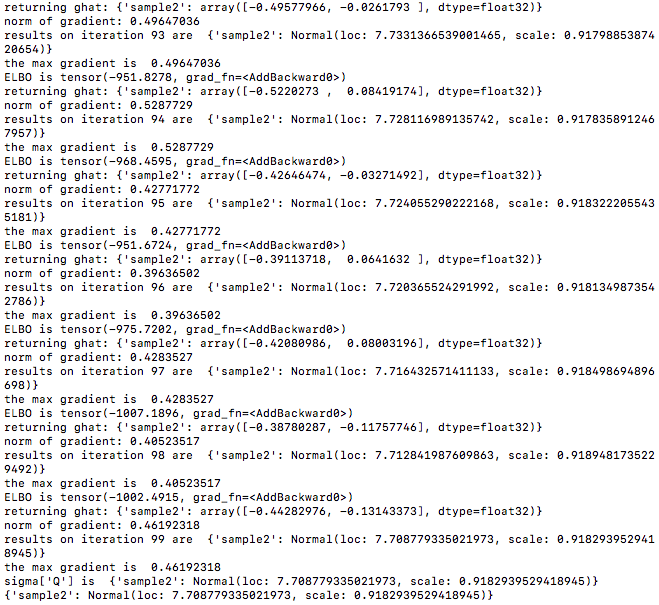
\includegraphics[scale=0.6]{p1_variational}
	\end{figure}
	
	\begin{figure}[h]
	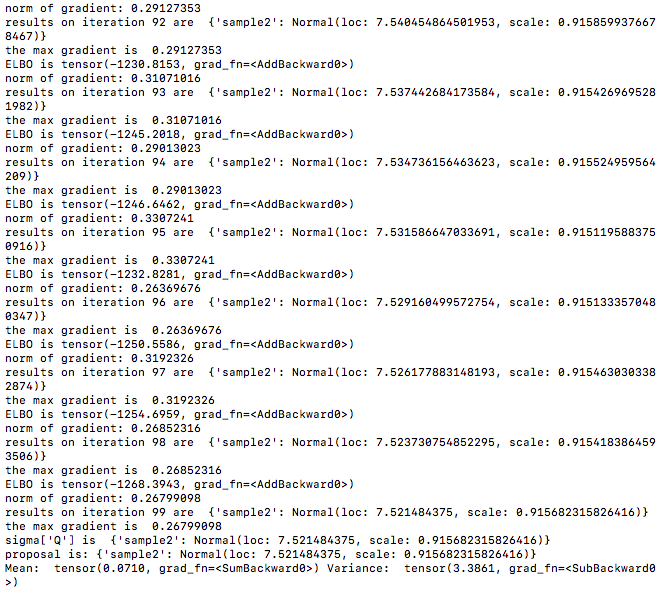
\includegraphics[scale=0.7]{program1}
	\end{figure}
	
	\newpage 
	But the sampled values look wrong:
	
	\begin{figure}[h]
	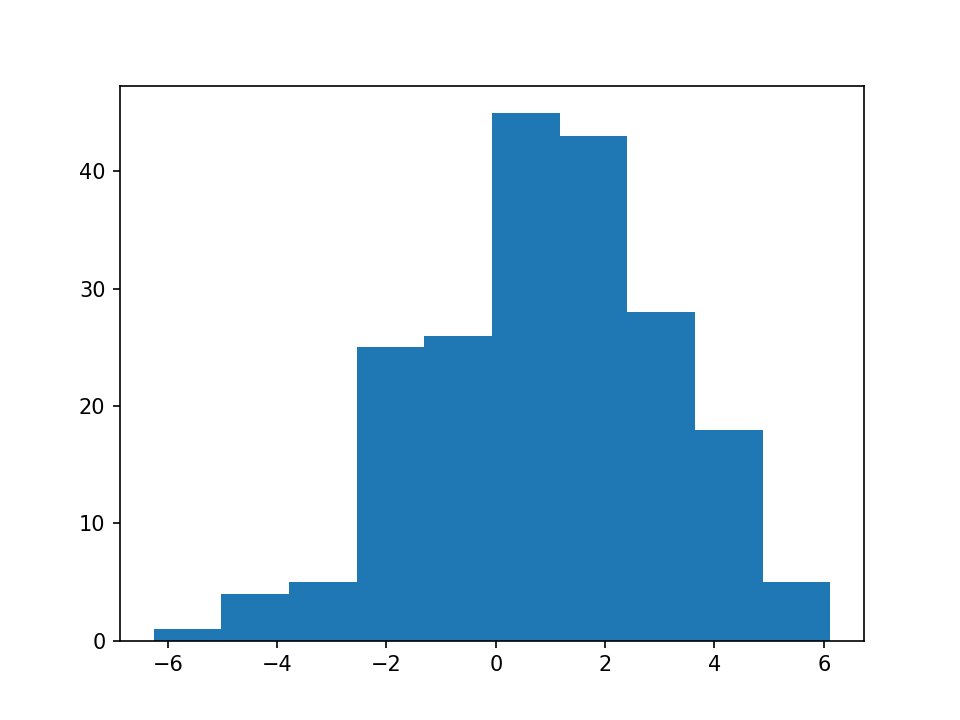
\includegraphics[scale=0.7]{p1histogram.png}
	\end{figure}
	


	\newpage
	

	
	\section{Program2}
		Again we can see that the optimized proposal is looking correct.
	\begin{figure}[h]
	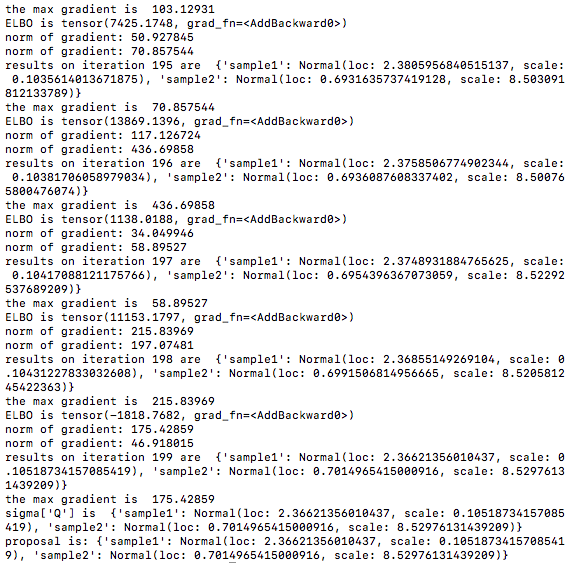
\includegraphics[scale=0.7]{p2proposal}
	\end{figure}
	
	\newpage
	
	\section{Program3}

	I have a bug that only affects program 3.
	
	\newpage
	
	\section{Program4}
	
	\begin{figure}[h]
	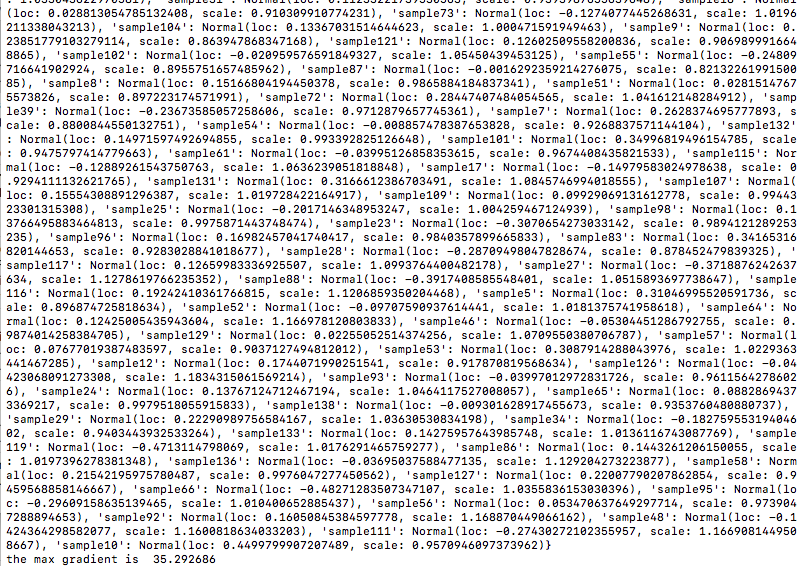
\includegraphics[scale=0.7]{p4proposal}
	\end{figure}
	\newpage
		
	\section{Program5}
		
	\begin{figure}[h]
	\end{figure}
	
	

	
	
	
	\section{Program3}
	
	
	
	

		

	
	
	
	
	
	
	\subsection{results}
	

	
	
	
	
	
	
		
	\newpage
	
	
	
	
%	\bibliography{research.bib}
%	\bibliographystyle{plain}
	
	
\end{document}